\chapter{Task}
In this dissertation we consider the problem of Edge-Level ML detection. This means, considering the Graph $G = (V, E)$ as in Definition \ref{financialGraph}, trying to learn a function \(f\) that, for each transaction $e \in E$, predicts its class. In particular we will consider two different settings. A binary classification where each edge is labeled as fraudulent or lecit and a multi-class classification where, in case of illicit transaction, we also predict the type of pattern, amongst the one described in Section \ref{mlpatterns}, it's involved in.

Formally we seek a function \(f\) that minimizes the error \(L(f)\) over a distribution \(\mathcal{D}\) of Graphs.
\begin{equation}
    \operatorname{argmin}_{f \in \mathcal{H}} \left\{L(f) \doteq \mathbb{E}_{(x,y) \sim \mathcal{D}} [l(f(x), y)]\right\}
\end{equation}
Practically there's no way to know \(\mathcal{D}\). Instead we will consider a dataset \(G_D = (V_D, E_D)\), where both nodes and edges are equipped with feature vectors and we will seek a function \(f\) that minimizes \(L(f)\) over this dataset computing the empirical risk:
\begin{equation}
    \operatorname{argmin}_{f \in \mathcal{H}} \left\{\hat{L}(f) \doteq \frac{1}{|E_D|} \sum_{e \in E_D} l(f(x_e), y_e)\right\}
\end{equation}
This is just the theoretical overview of the problem. In Chapter \ref{approaches} we will provide more insights on how to define the hypothesis space \(\mathcal{H}\) and the loss function \(l\). 

As mentioned in Chapter \ref{ethics_privacy_regulations}, the strict privacy regulations that governs the financial world, makes it hard to find real-world datasets. In this dissertation, for the reasons explained in Section \ref{patterns}, we will use the synthetic dataset \textit{IBM AMLSim}. This is perfect for our scope, since it provides edge lables for both binary and multiclass classification.

\section{Dataset description}
The IBM AMLSim dataset comes in 6 different versions.
\begin{itemize}
    \item HI-Small
    \item HI-Medium
    \item HI-Large  
    \item LO-Small
    \item LO-Medium
    \item LO-Large
\end{itemize}
Where HI (High) and LO (Low) indicate the frequency of illicit transactions and the suffixes Small, Medium and Large indicate the size of the dataset. Figure \ref{fig:datasetstats} shows the differences between the 6 datasets.
\begin{figure}
    \centering
    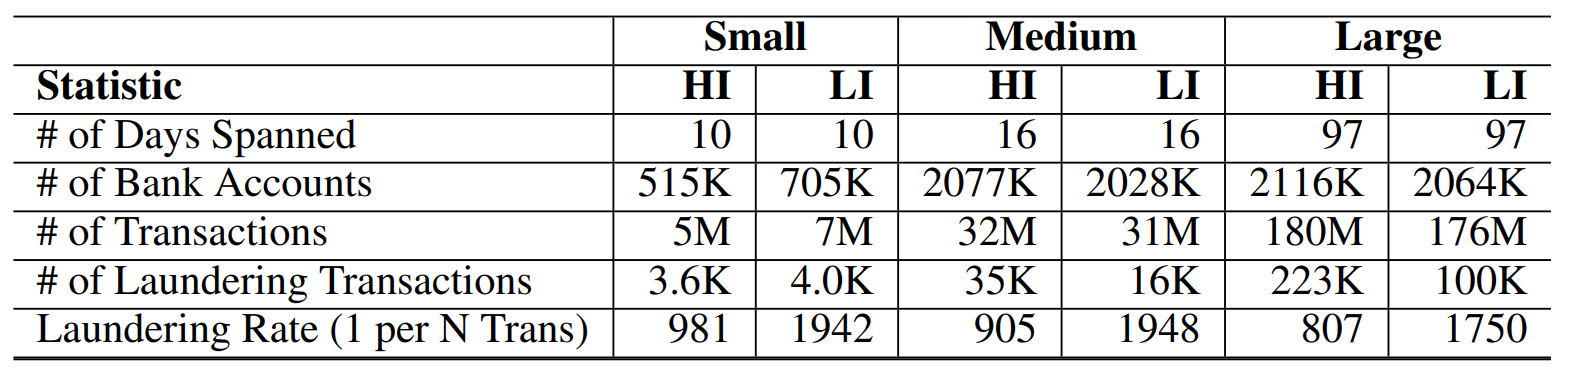
\includegraphics[width=1.0\textwidth]{IMG/dataset.png}
    \caption{IBM AMLSim datasets statistics \cite{AMLWorld}}
    \label{fig:datasetstats}
\end{figure}

In this work we will use the HI-Small version. Bigger datasets would of course garantee a better generalization and accuracy but, for hardware and time constraint, it would be impossible to train the models on such graphs. That begin said, we belive that the obtained results are good enough to understand how the models would perform in a real world scenario.

The HI-Small dataset is composed of 3 different files:
\begin{itemize}
    \item \texttt{HI-Small\_account.csv}, contains 518,581 accounts toghether with their features:
    \begin{itemize}
        \item \textit{Entity ID}: The ID of the account;
        \item \textit{Entity Name}: The name of the account;
        \item \textit{Bank Name}: The name of the bank holding the account; 
        \item \textit{Bank ID}: The ID of the bank holding the account;
        \item \textit{Account Number}: The number of the account;    
    \end{itemize}
    Figure \ref{fig:accountshead} shows some examples of account records.
    \item \texttt{HI-Small\_Trans.csv}, contains transactions features and binary labels:
    \begin{itemize}
        \item \textit{Timestamp}: The timestamp of the transaction;
        \item \textit{From Bank}: The ID of the sending bank;
        \item \textit{From Account}: The ID of the sending account;
        \item \textit{To Bank}: The ID of the receiving bank;
        \item \textit{To Account}: The ID of the receiving account;
        \item \textit{Amount Received}: The amount of money received by the recipient;
        \item \textit{Receiving Currency}: The currency of the received amount (USD, EUR, etc.);
        \item \textit{Amount Paid}: The amount of money paid by the sender;
        \item \textit{Payment Currency}: The currency of the paid amount;
        \item \textit{Payment Format}: The format/method of the payment;
        \item \textit{Is Laundering}: Binary label indicating whether the transaction is illicit;
        \item \textit{src}: Source node identifier;
        \item \textit{dst}: Destination node identifier;
    \end{itemize}
    Figure \ref{fig:transhead} shows some examples of transaction records.
    \item \texttt{HI-Small\_Patterns.txt}, lists the edges that are involved in ML activities toghether with the type of pattern they are involved in (multiclass labels).
    Examples of the 8 differt types of ML patterns in IBM AMLSim are shown in Figure \ref{fig:patternsIBM}.
\end{itemize}
\begin{figure}
    \centering
    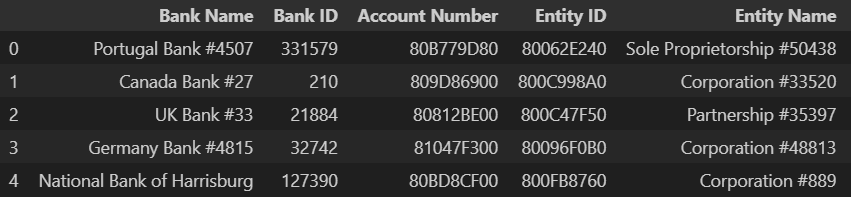
\includegraphics[width=1.0\textwidth]{IMG/accounts_head.png}
    \caption{IBM AMLSim account records}
    \label{fig:accountshead}
\end{figure}
\begin{figure}
    \centering
    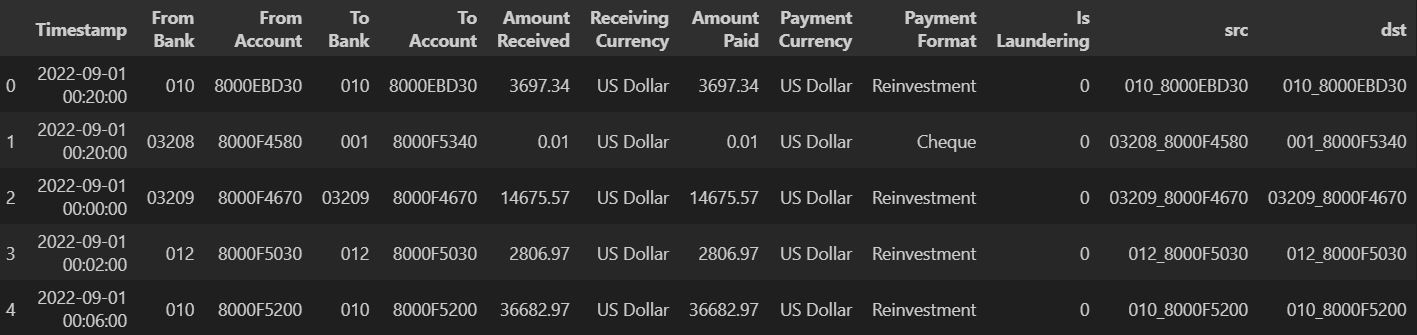
\includegraphics[width=1.0\textwidth]{IMG/trans_head.png}
    \caption{IBM AMLSim transaction records}
    \label{fig:transhead}
\end{figure}
\begin{figure}
    \centering
    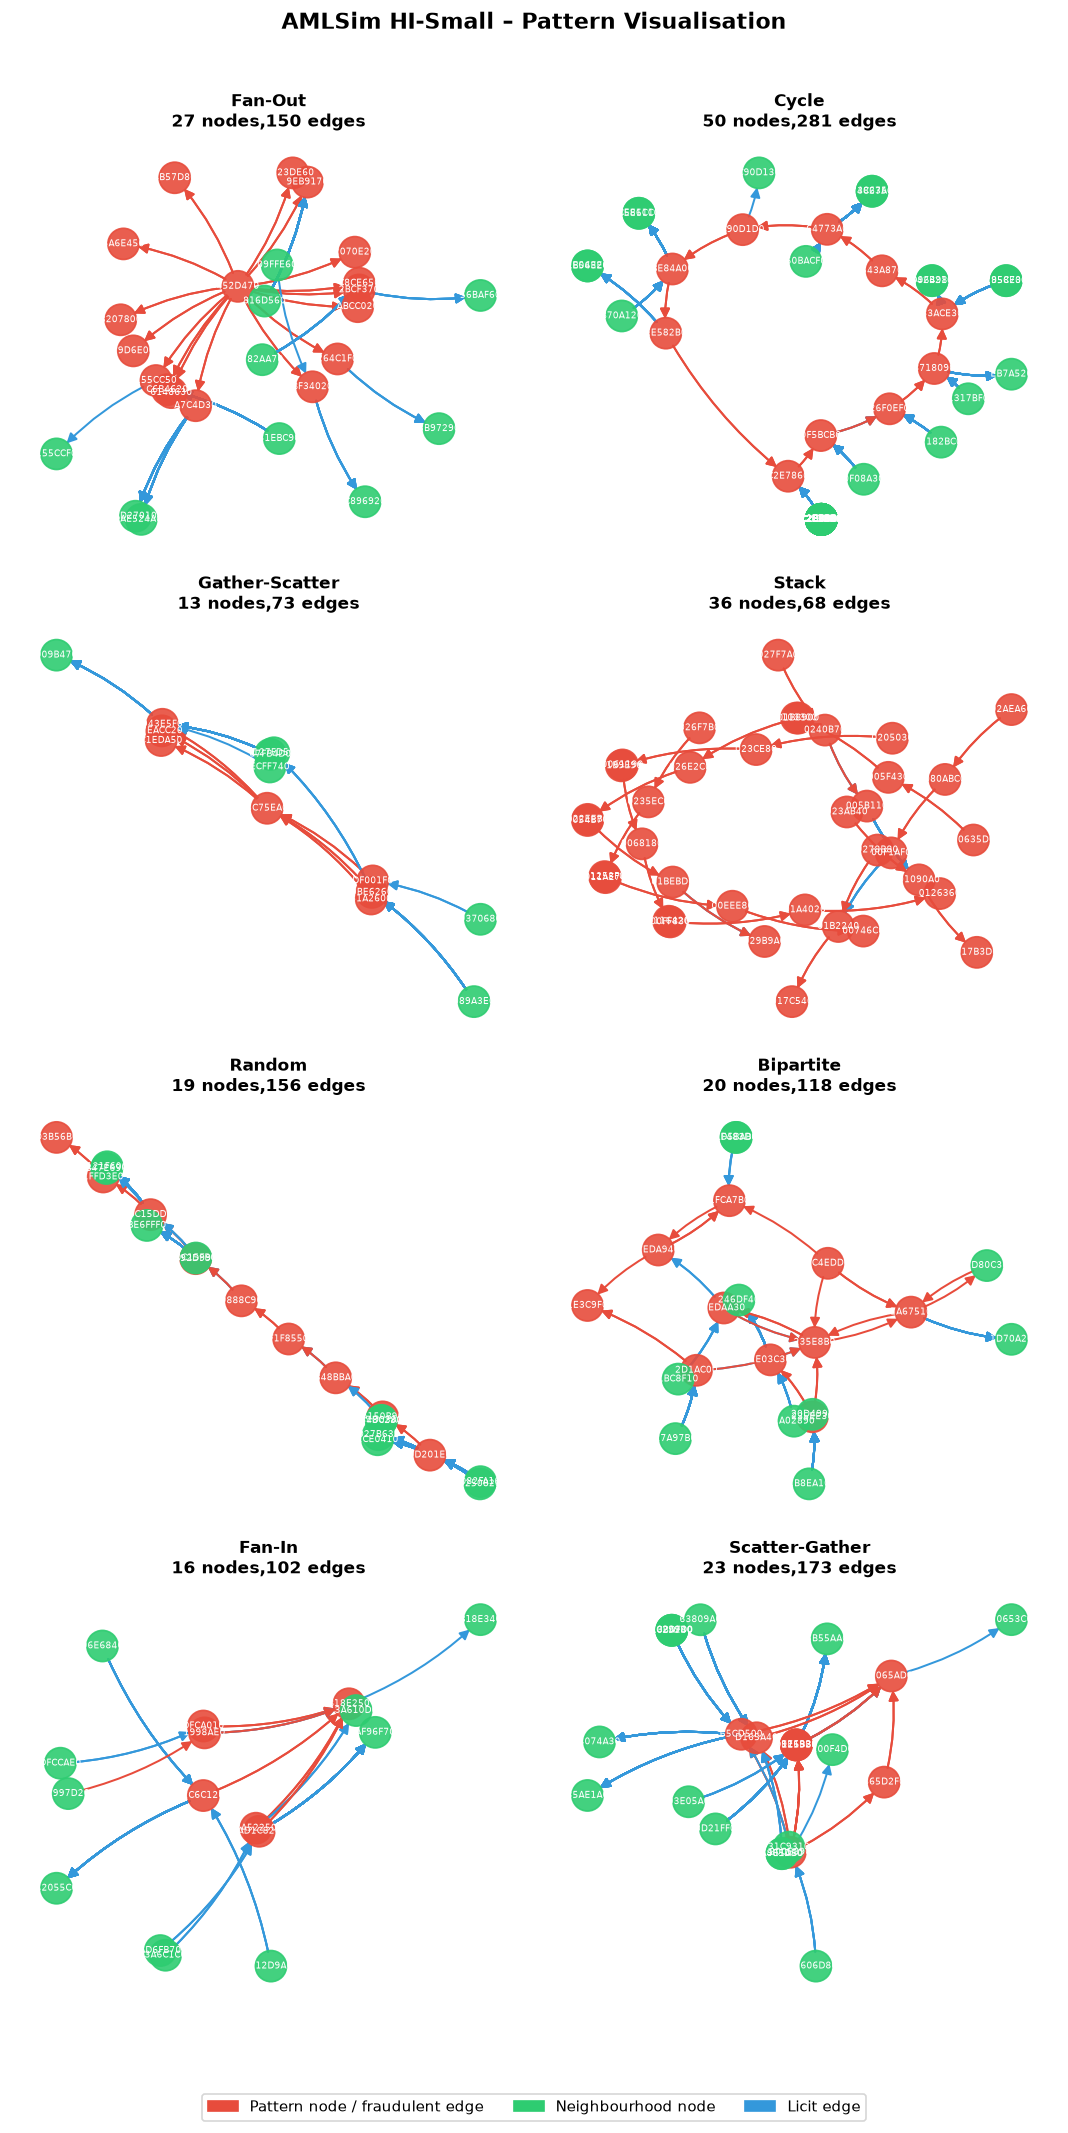
\includegraphics[width=0.76\textwidth]{IMG/patterns.png}
    \caption{IBM AMLSim patterns examples}
    \label{fig:patternsIBM}
\end{figure}
\section{Features analysis}
In this section we provide a detailed analysis of the edges and nodes features distributions. Before diving into that we first take a look at the distribution of the labels in the dataset. There are \(5,177\) illicit transactions over a total of \(5,078,345\) Edges.
Figure \ref{fig:patterns_distr}, provides the distribution of the multiclass label (type of pattern) over the fraudulent edges. It's important to notice that this information is provided only for \(3,149\) out of the \(5,177\) illicit transactions.
\begin{figure}
    \centering
    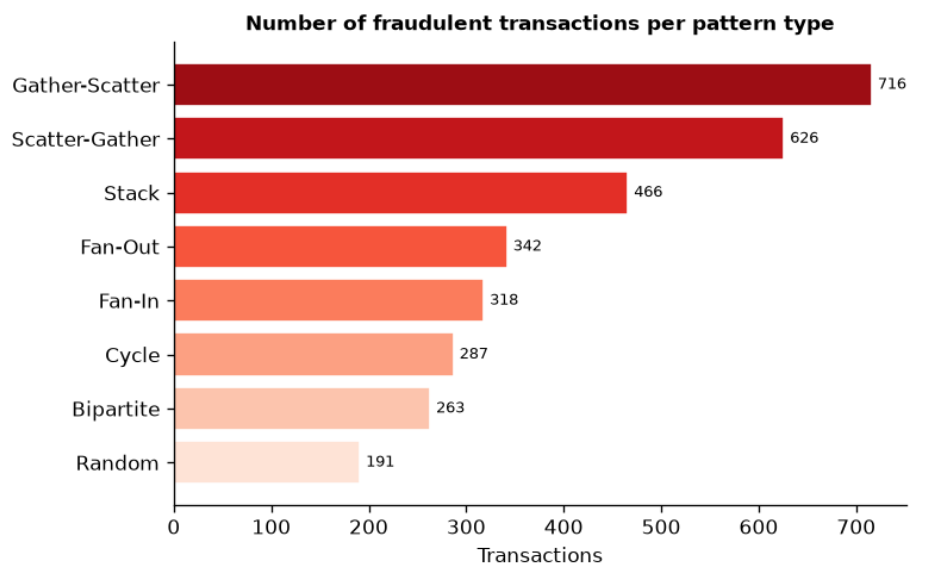
\includegraphics[width=0.8\textwidth]{IMG/patterns_distr.png}
    \caption{IBM AMLSim patterns distribution over fraudulent edges}
    \label{fig:patterns_distr}
\end{figure}

We now procede by analyzing the edge features. First, we notice that \textit{Amount Received} and \textit{Amount Paid} are almost identical. From Figure \ref{fig:amounttrans} we can see that fraudulent trasnactions have the tendency to be bigger than lecit ones.

Continuing our analysis on edge features, we notice that the most common currency is USD for both fraudulent and licit transactions; most of the currencies have a similar proportion distribution from both fraudulent and licit transactions. From Figure \ref{fig:currencytrans} we can see that there are two exceptions: Shekel, which is more prevalent in licit transactions, and Saudi Riyal, which is significantly more prevalent in fraudulent transactions. It's important to notice that the graph shows the proportion of each currency with respect to the total number of transactions in each class; Since there are way more licit than fraudulent transactions, having similar distributions means that, for every type of currency, licit transactions still represent the vast majority.

Considering now the payment formats, by looking at Figure \ref{fig:paymentformats} we notice that ACH transactions are more frequently used for fraudulent transactions compared to other methods.

The last edge feature is \textit{Timestamp}. Since working with timestamps can be tricky, we decided to extract to categorical features representing the hour of the day and the day of the week (Figures \ref{fig:hourday}). Normally we would have also considered the week of the year and the year itself but, since IBM AMLSim Small only covers the span of a week, it would be irrelevant. That being said, it's important to mention that directly working with timestamps, albeit tricky, could lead to a more precise detection [Chapter \ref{futureDirections}]. 
\begin{figure}
    \centering
    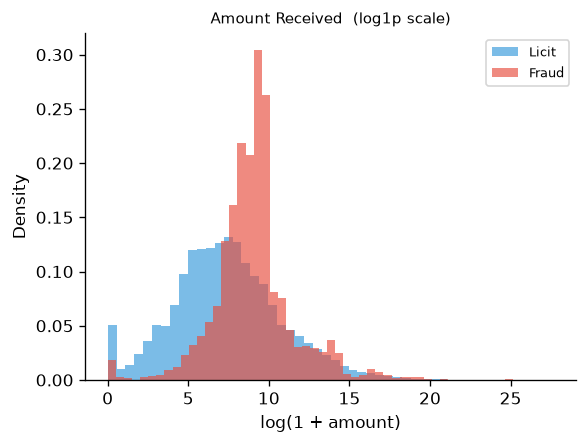
\includegraphics[width=0.8\textwidth]{IMG/amount.png}
    \caption{IBM AMLSim amounts distribution}
    \label{fig:amounttrans}
\end{figure} 
\begin{figure}
    \centering
    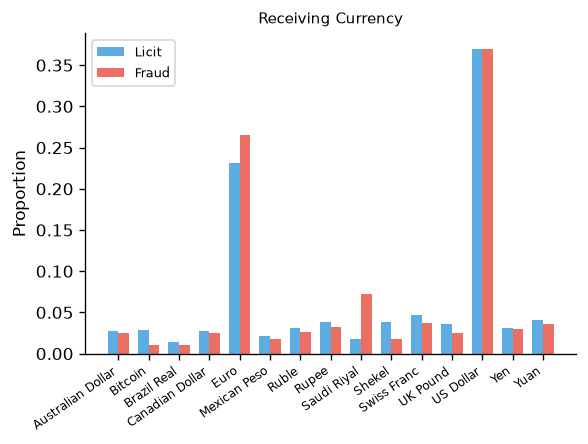
\includegraphics[width=0.8\textwidth]{IMG/currencies.png}
    \caption{IBM AMLSim currencies distribution}
    \label{fig:currencytrans}
\end{figure} 
\begin{figure}
    \centering
    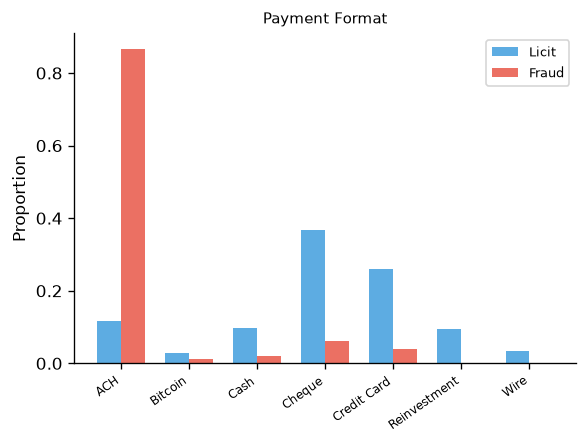
\includegraphics[width=0.8\textwidth]{IMG/format.png}
    \caption{IBM AMLSim payment formats distribution}
    \label{fig:paymentformats}
\end{figure} 
\begin{figure}
    \centering
    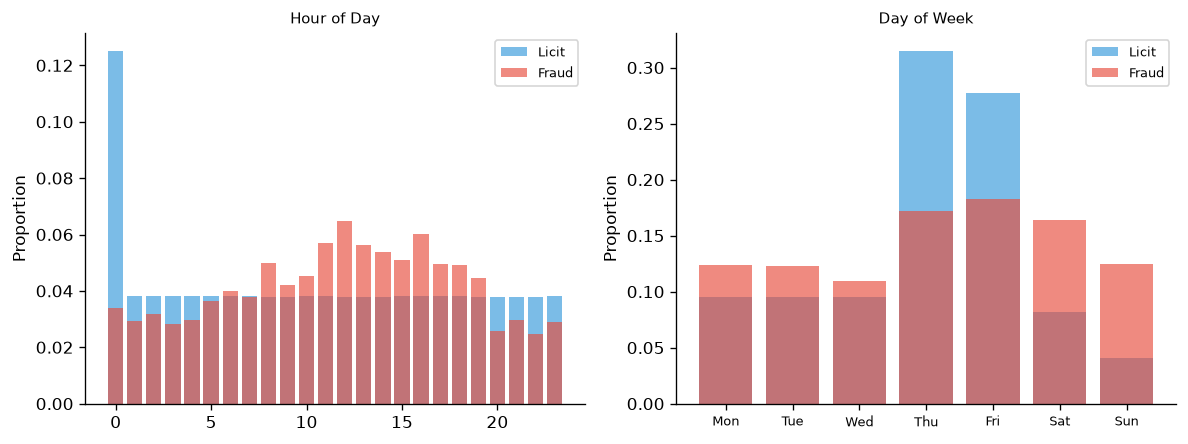
\includegraphics[width=0.8\textwidth]{IMG/hourday.png}
    \caption{IBM AMLSim hour and day of the week distributions}
    \label{fig:hourday}
\end{figure} 

Finally we take a look at the Node features. The only intresting one is \textit{Bank Name}, Figure \ref{fig:bank} shows the distribution of licit and illicit nodes over the 10 biggest banks.
\begin{figure}
    \centering
    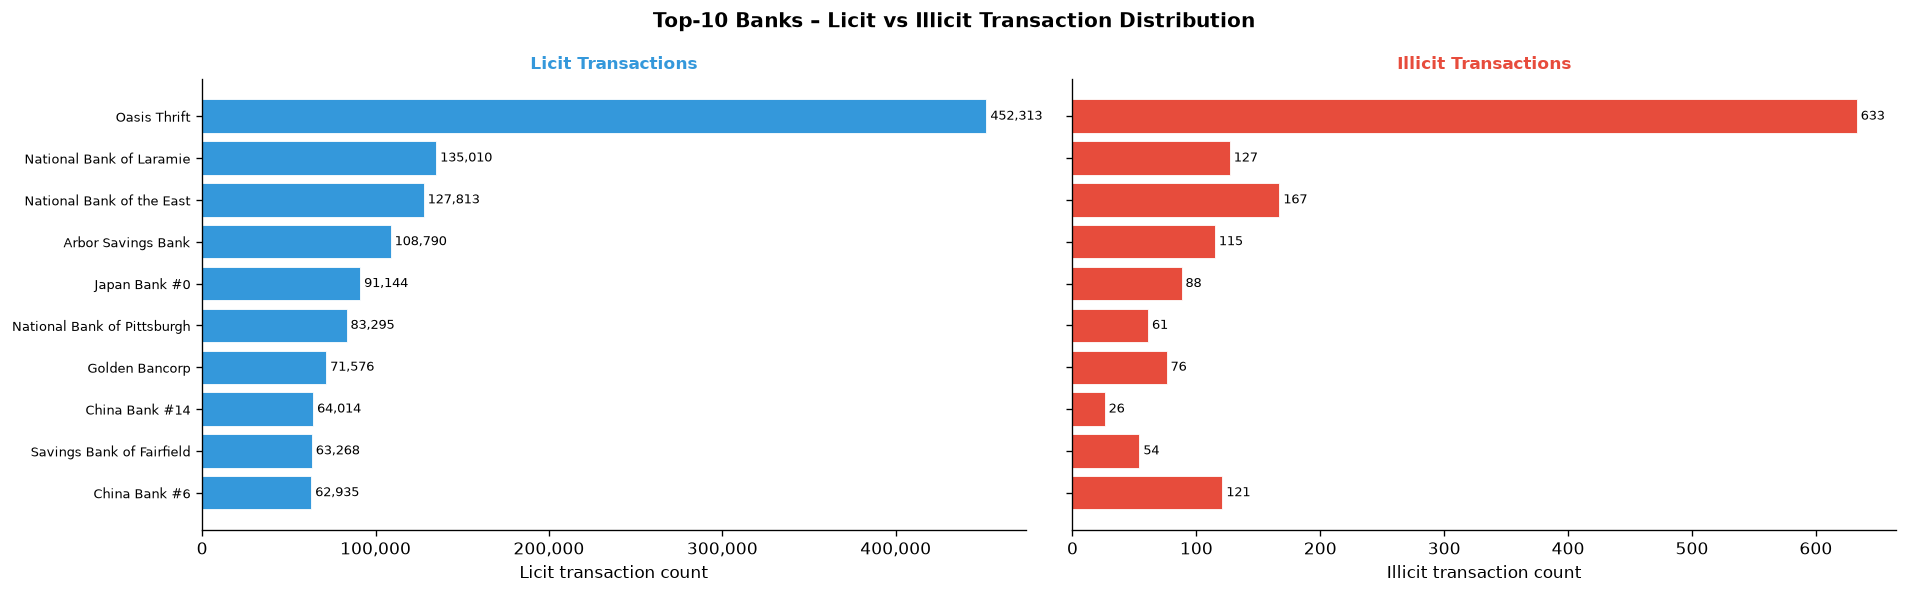
\includegraphics[width=0.8\textwidth]{IMG/banks.png}
    \caption{IBM AMLSim banks distribution}
    \label{fig:bank}
\end{figure} 